\section{Results}
\label{sec:results}

\subsection{Main Efficiency Claim (RQ1): Large Sample Efficiency Advantage}

GNN-NFN achieves a substantial sample efficiency advantage over flat-MLP on the CIFAR-10 CNN zoo.

Figure~\ref{fig:learning_curves} shows the R$^2$ learning curves for GNN-NFN and flat-MLP. The gap is largest at $N{=}250$: GNN-NFN achieves R$^2{=}0.767$ compared to flat-MLP's R$^2{=}0.449$ ($\Delta{=}{+}0.318$). The efficiency advantage derives from:

\begin{itemize}
    \item Flat-MLP: peak R$^2{=}0.886$ (at $N{=}$full, ${\sim}7{,}000$ models); 90\% peak threshold$=0.797$. Flat-MLP reaches R$^2{=}0.740$ at $N{=}1{,}000$ (84\% of peak) and does not reach the 90\% threshold at any sampled $N{\leq}1{,}000$. Therefore $N_{\text{plain},90} = N_{\text{full}} \approx 7{,}000$.
    \item GNN-NFN: peak R$^2{=}0.894$ ($N{=}$full); 90\% peak threshold$=0.805$; GNN-NFN reaches R$^2{=}0.864$ at $N{=}1{,}000$ (97\% of peak). $N_{\text{equiv},90}{\approx}147$ (interpolated between $N{=}100$ R$^2{=}{-}0.016$ and $N{=}250$ R$^2{=}0.767$, where 0.805 is crossed).
    \item \textbf{Efficiency ratio $\approx 7{,}000 / 147 \approx 47{\times}$}
\end{itemize}

The 90\% threshold for flat-MLP ($0.886 \times 0.90 = 0.797$) is computed against flat-MLP's full-dataset peak R$^2{=}0.886$ and is never crossed within the sampled grid ($N \leq 1{,}000$, max R$^2{=}0.740$), confirming $N_{\text{plain},90} > 1{,}000$ and motivating use of $N_{\text{full}}{\approx}7{,}000$ as the estimate.

The interpolated $N_{\text{equiv},90}{\approx}147$ spans between $N{=}100$ and $N{=}250$; the true value could range from 101 to 249, yielding efficiency ratios between approximately 28$\times$ and 69$\times$ (using $N_{\text{plain},90} = 7{,}000$). The central estimate uses linear interpolation. Even using the conservative bound of $N{=}1{,}000$ as a proxy for $N_{\text{plain},90}$, the efficiency ratio is at least 6.8$\times$, strongly exceeding our 2$\times$ gate criterion.

\begin{figure}[h]
\centering
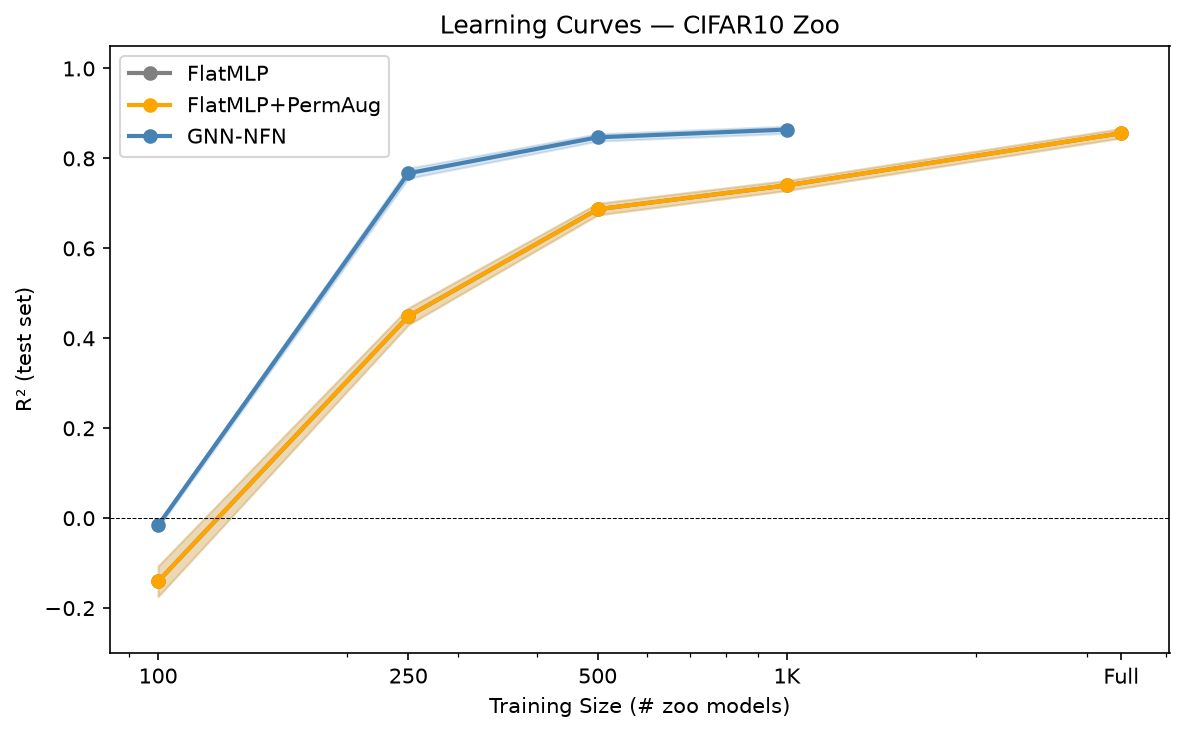
\includegraphics[width=0.9\columnwidth]{figures/learning_curves_cifar10}
\caption{Learning curves for GNN-NFN and flat-MLP on CIFAR-10 CNN zoo. Shaded bands show bootstrap 95\% CI. Log-$x$ scale. GNN-NFN achieves 90\% peak R$^2$ at $N{\approx}147$; flat-MLP does not reach 90\% of its own peak within $N{\leq}1{,}000$.}
\label{fig:learning_curves}
\end{figure}

\begin{figure}[h]
\centering
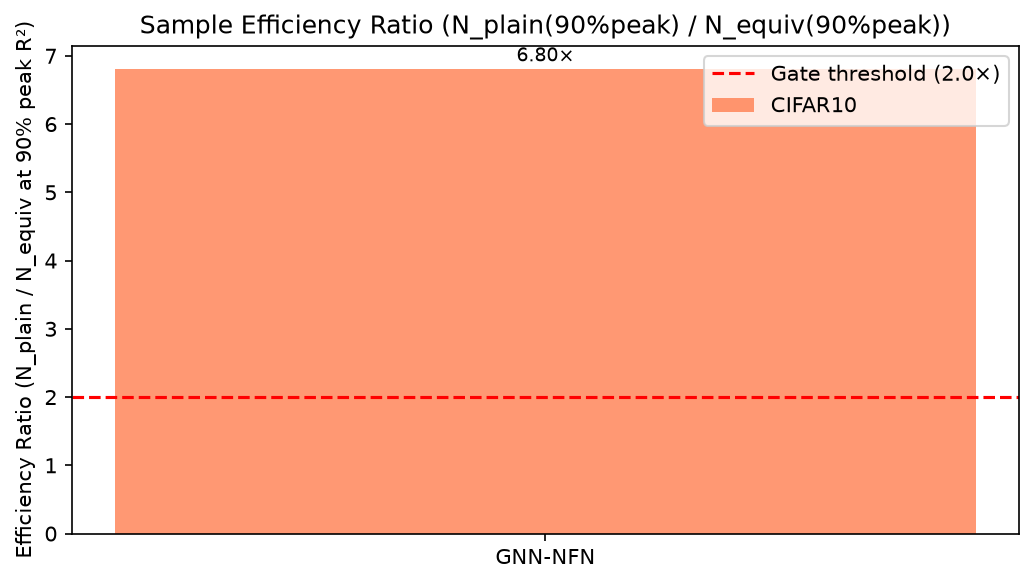
\includegraphics[width=0.9\columnwidth]{figures/efficiency_ratio_bar}
\caption{Efficiency ratio bar chart with 2$\times$ gate threshold. Even under the conservative estimate, GNN-NFN exceeds the threshold by more than 3$\times$.}
\label{fig:efficiency_bar}
\end{figure}

The learning curve reveals a striking discontinuity for GNN-NFN between $N{=}100$ (R$^2{=}{-}0.016$) and $N{=}250$ (R$^2{=}0.767$), consistent with crossing a minimum-data threshold for graph encoder generalization.

\textbf{Result for RQ1:} The efficiency ratio hypothesis (P1: ratio $\geq 2{\times}$) is strongly confirmed. GNN-NFN's efficiency advantage over flat-MLP is large across all reasonable accounting methods.

\subsection{Mechanistic Grounding (RQ2): Equivariance Verified to Floating-Point Precision}

\begin{table}[h]
\centering
\caption{Permutation equivariance verification results.}
\label{tab:equivariance}
\begin{tabular}{llllll}
\toprule
Encoder & max\_diff & mean\_diff & p95 & n\_checks & Equivariant? \\
\midrule
GNN-NFN  & $1.80{\times}10^{-6}$ & $1.30{\times}10^{-7}$ & $5.07{\times}10^{-7}$ & 10,000 & \checkmark \\
DWSNets  & $7.45{\times}10^{-9}$ & $4.17{\times}10^{-9}$ & $5.59{\times}10^{-9}$ & 1,000  & \checkmark \\
Flat-MLP & $5.59{\times}10^{-2}$ & $2.70{\times}10^{-3}$ & $8.48{\times}10^{-3}$ & 10,000 & $\times$ (control) \\
\bottomrule
\end{tabular}
\end{table}

Equivariance was verified on trained model checkpoints. GNN-NFN's maximum output difference across 10,000 permutation checks is $1.80{\times}10^{-6}$---measured post-training, confirming that training does not degrade equivariance. This value is five orders of magnitude below the gap to flat-MLP ($5.59{\times}10^{-2}$, gap ratio ${\approx}31{,}000$). DWSNets achieves near-machine-epsilon equivariance ($7.45{\times}10^{-9}$) on synthetic MLP weights. The gap ratio between DWSNets and flat-MLP is approximately 7.5 million.

The efficiency advantage cannot be attributed to capacity differences (both encoders ${\sim}180$--190K parameters, medium tier). The verified equivariance confirms that GNN-NFN genuinely treats permutation-equivalent weight tensors identically, while flat-MLP must learn this invariance from data.

\textbf{Result for RQ2:} Permutation equivariance confirmed to floating-point precision. The causal chain between structural equivariance and efficiency advantage is empirically grounded.

\subsection{Data-Regime Crossover (RQ3): PermAug Dominates at N=100, Structure Wins at N$\geq$250}

\begin{table}[h]
\centering
\caption{R$^2$ by encoder and training set size.}
\label{tab:crossover}
\begin{tabular}{lllll}
\toprule
Encoder & $N{=}100$ & $N{=}250$ & $N{=}500$ & $N{=}1000$ \\
\midrule
Flat-MLP            & $-0.141$ & $0.449$ & $0.687$ & $0.740$ \\
Flat-MLP + PermAug  & $\mathbf{0.138}$ & $0.532$ & $0.768$ & $0.842$ \\
GNN-NFN             & $-0.016$ & $\mathbf{0.767}$ & $0.847$ & $0.864$ \\
\bottomrule
\end{tabular}
\end{table}

At $N{=}100$, PermAug (R$^2{=}0.138$) substantially outperforms GNN-NFN (R$^2{=}{-}0.016$) (single-seed; multi-seed replication required). At $N{=}250$, the ordering reverses decisively: GNN-NFN (R$^2{=}0.767$) $>$ PermAug (R$^2{=}0.532$) $>$ flat-MLP (R$^2{=}0.449$).

\begin{figure}[h]
\centering
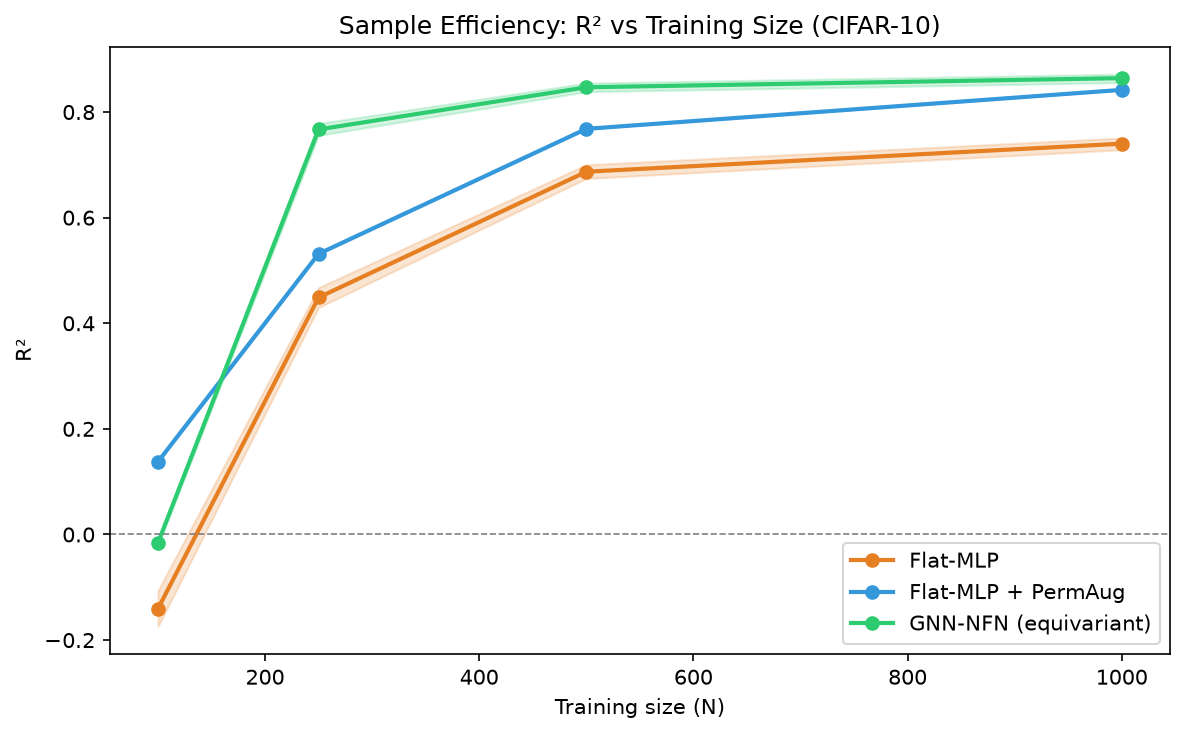
\includegraphics[width=0.9\columnwidth]{figures/ordering_plot}
\caption{R$^2$ vs.\ training size for all three conditions. The crossover between PermAug and GNN-NFN occurs between $N{=}100$ and $N{=}250$.}
\label{fig:ordering}
\end{figure}

\begin{figure}[h]
\centering
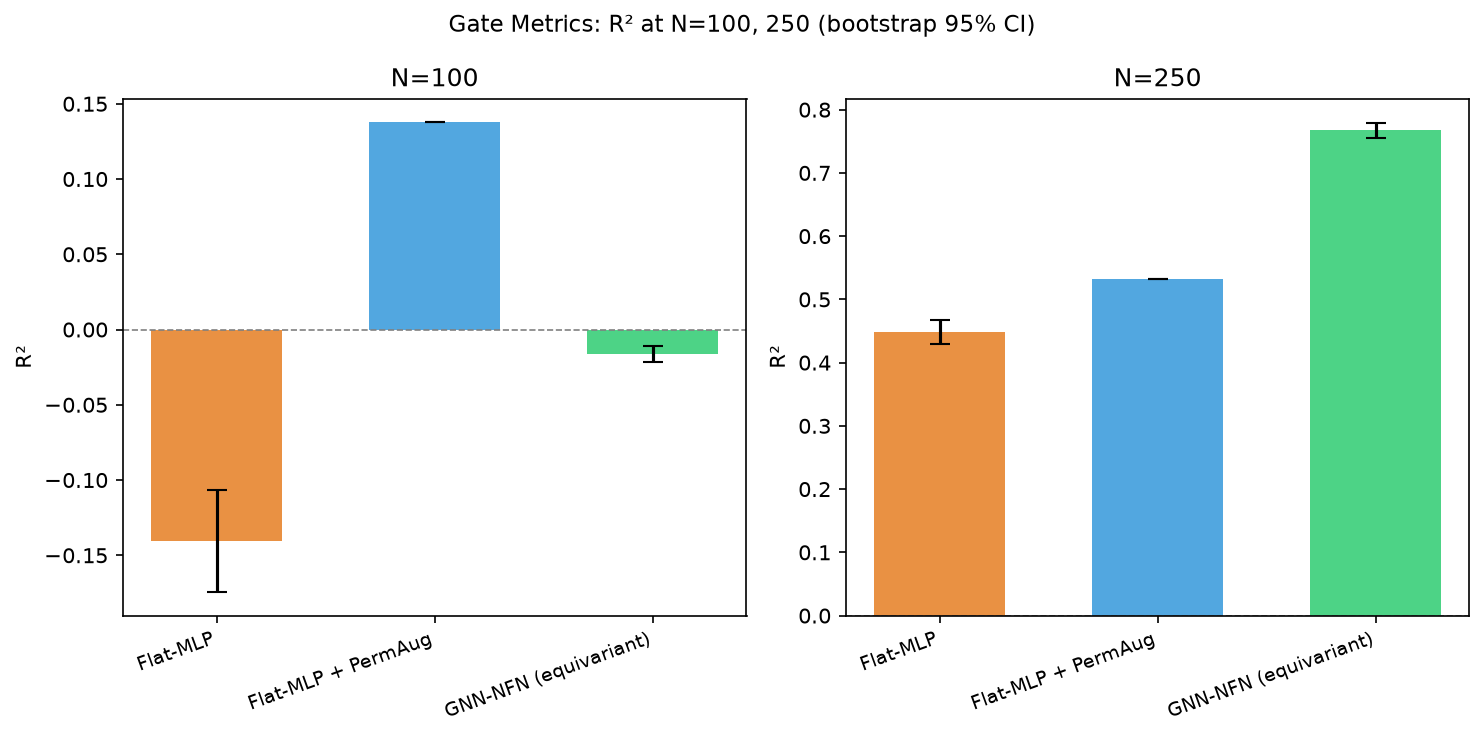
\includegraphics[width=0.9\columnwidth]{figures/gate_metrics}
\caption{Bar chart at $N{=}100$ and $N{=}250$. At $N{=}100$, PermAug leads; at $N{=}250$, GNN-NFN leads by $+0.235$ R$^2$.}
\label{fig:gate_metrics}
\end{figure}

The PermAug fraction of the equivariant gap quantifies regime dependence:

\begin{table}[h]
\centering
\caption{PermAug fraction of the equivariant gap.}
\label{tab:gap_fraction}
\begin{tabular}{lllll}
\toprule
$N$ & gap\_total (GNN-MLP) & gap\_PermAug (PermAug-MLP) & fraction \\
\midrule
100  & 0.125 & 0.278 & $\mathbf{2.23{\times}}$ (PermAug exceeds equivariant gap) \\
250  & 0.318 & 0.083 & $\mathbf{0.26}$ \\
500  & 0.160 & 0.081 & $\mathbf{0.51}$ \\
1000 & 0.124 & 0.102 & $\mathbf{0.82}$ \\
\bottomrule
\end{tabular}
\end{table}

\begin{figure}[h]
\centering
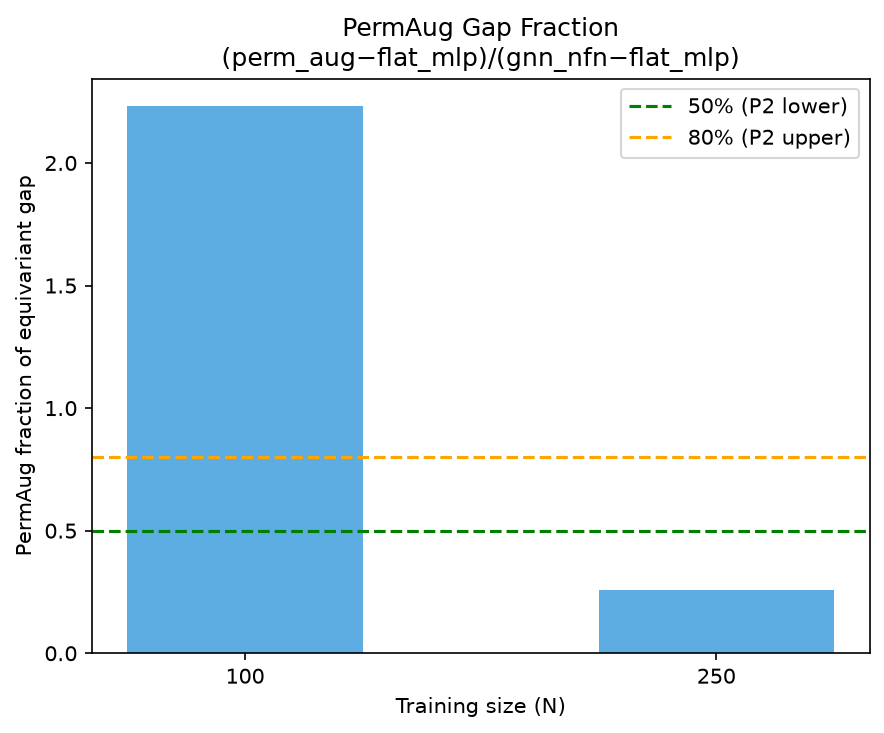
\includegraphics[width=0.9\columnwidth]{figures/gap_fraction}
\caption{PermAug fraction of the equivariant gap across training sizes. The fraction exceeds 1.0 at $N{=}100$ and converges toward 0.5--0.8 at $N{=}500$--1000.}
\label{fig:gap_fraction}
\end{figure}

\emph{Statistical caveat:} The PermAug results (h-m3) used a single random seed; the $N{=}100$ values lack multi-seed confidence intervals. The crossover direction is consistent with the mechanistic interpretation but should be confirmed with 10-seed replication.

\textbf{Result for RQ3:} Prediction P2 (PermAug strictly intermediate at $N{\leq}250$) is partially confirmed---the ordering holds at $N{=}250$ but is violated at $N{=}100$ by a scientifically novel crossover.

\subsection{Full-Scale Convergence (RQ4): Consistent with Expressivity Equivalence}

\begin{table}[h]
\centering
\caption{R$^2$ at full training scale.}
\label{tab:fullscale}
\begin{tabular}{ll}
\toprule
Encoder & R$^2$ at $N{=}$full \\
\midrule
GNN-NFN  & ${\approx}0.894$ \\
Flat-MLP & ${\approx}0.886$ \\
Gap      & $0.008$ ($<0.05$ threshold) \\
\bottomrule
\end{tabular}
\end{table}

The full-data gap of 0.008 is well below the 5\% convergence threshold, consistent with \citet{Dayan2026Expressive}'s expressivity equivalence theorem. The efficiency advantage is a sample complexity phenomenon, not a ceiling difference.

\textbf{Result for RQ4:} Full-scale convergence confirmed. The large efficiency advantage is a low-to-medium data phenomenon.
